\documentclass[UTF8]{ctexart}

\usepackage{subfiles}  

%下面的语句, 引入你的头部设置文件
\usepackage{C:/phpStorm_proj/02_myself_ID_EGO/+100_latex_all_math_sel/myPreamble} 
%必须是绝对路径,才能让各个tex在单独编译时使用到

\title{文件名}


%---------------------------------


\begin{document}
	\tableofcontents % 生成目录
	\date{} % 若不写这句, 则默认也会渲染出日期, 所以我们要手动赋空值
	\maketitle  %这行代码, 让你前面的 title, author, date生效
	
	
	
	\part{几何概型}
	
	
	\section{几何概型 geometric models of probability}
	
	
	几何概型 geometric models of probability, 即这类概率问题, 能够转换成用``几何问题"来求解. \\
	
	\begin{myEnvSample}
		有甲乙两人, 相约在 6-7点见面 (其实这个具体的时间点也是个障眼法, 只要在1个小时的区间就行). 先到者, 最多等对方15分钟, 然后就离开了.
		
		甲乙两人, 在这1小时内的任意时刻, 都可能到达.
		
		问, 他们能相见的概率是多少? \\
		
		我们令 
		
		- 事件A : 表示两人见到了面 \\
		- x : 表示甲到达的时间点 \\
		- y : 表示乙到达的时间点 \\
		
		他们要能见到面, 即 $|y-x| \leq 15$分钟. 那么这就有两种可能性: \\
		-  甲先到. 即 $x \leq y$ (甲来到的时间点x, 比乙来到的时间点y 要小 (早)), 即 $ y-x \leq 15$ \\
		-  乙先到. 即 $y \leq x$, 即 $ x-y \leq 15$ \\	
		
		这两组不等式, 能用函数图形来表示出来, 如下图. x和y轴上的60, 分别代表两人的1小时区间(60分钟) . 中间的交集区域, 就是两人可以见到面的时间段. \\
		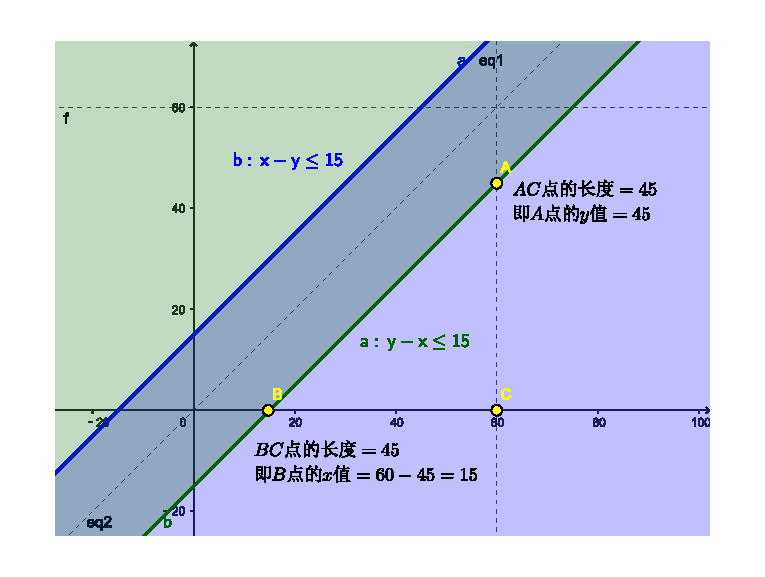
\includegraphics[width=0.9\textwidth]{/0083.pdf} \\
		
		显然, 这就是求几何面积的问题. \\
		
		即: $
		\text{P}\left( \text{A} \right) =\frac{60\cdot 60-\overset{\text{上面的``边长为45"的三角形的面积}}{\overbrace{\frac{45\cdot 45}{2}}}-\overset{\text{下面的``边长为45"的三角形的面积}}{\overbrace{\frac{45\cdot 45}{2}}}}{\underset{\text{即``边长为60分钟"的矩形}}{\underbrace{60\cdot 60}}}=0.4375
		$
	\end{myEnvSample} 
	\vspace{1em} 
	
	
	
	\begin{myEnvSample}
		(法国)布丰(1707-1788) 投针 Buffon's needle problem. \\
		说: 有两条平行的直线, 相聚为 D(distance), 距离单位不重要. 你哪一个针 (长度为 L (length), $L<D$), 随机地投向针. 问: 针与那两条平行直线 相交的概率是? \\
		
		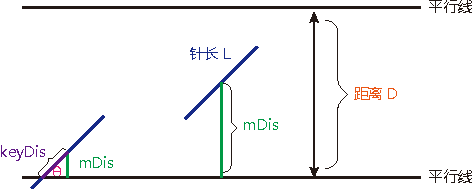
\includegraphics[width=0.6\textwidth]{/0086.pdf} \\
		
		思路: 针投上去后的位置状态, 是由两个参数决定的: \\
		(1) 针的中点, 距离``最近那根直线"的最短距离. ← 该距离用变量 mDis (midpoint distance)来表示. \\
		(2) 针倾斜的位置, 与直线的夹角. ← 我们用变量 $\theta$ 来表示.  \\
		用上面这两个变量, 我们能分别作为 x轴(表示 $\theta$ 变量) 和 y轴(表示 mDis变量), 来画出函数图像. \\
		
		针投出后, 所有可能的状态, 其全集就是: \\
		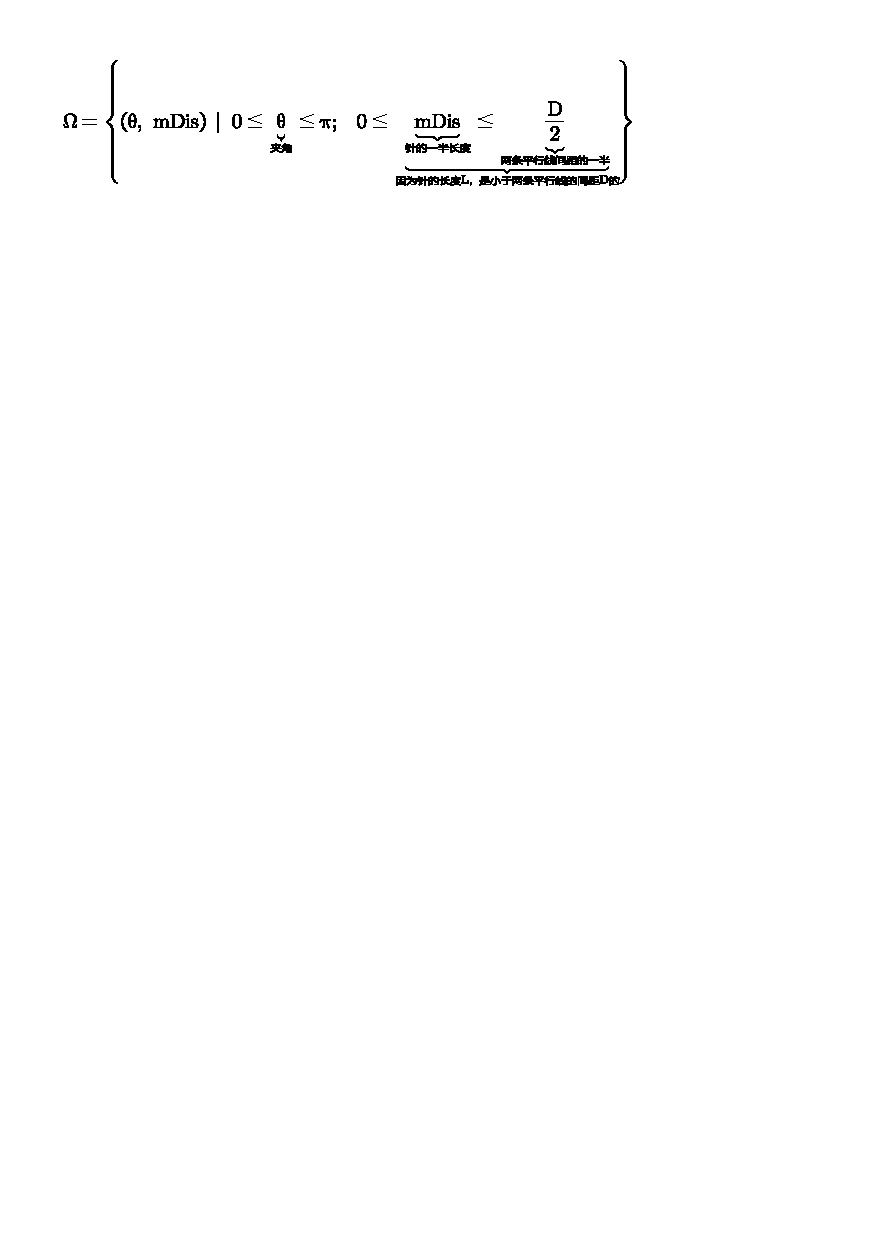
\includegraphics[width=0.8\textwidth]{/0084.pdf} \\
		
		那么, 什么状态下, ``针"就与``直线"相交了呢? -- 当``从针的中点(沿着针的身体走)到直线"的距离 (下面用变量 keyDis (key distance) 来表示这个距离) $\leq$ 针的一半长度时. 它们就相交了. 否则, 它们就不想交. \\
		即, 就有: \\	
		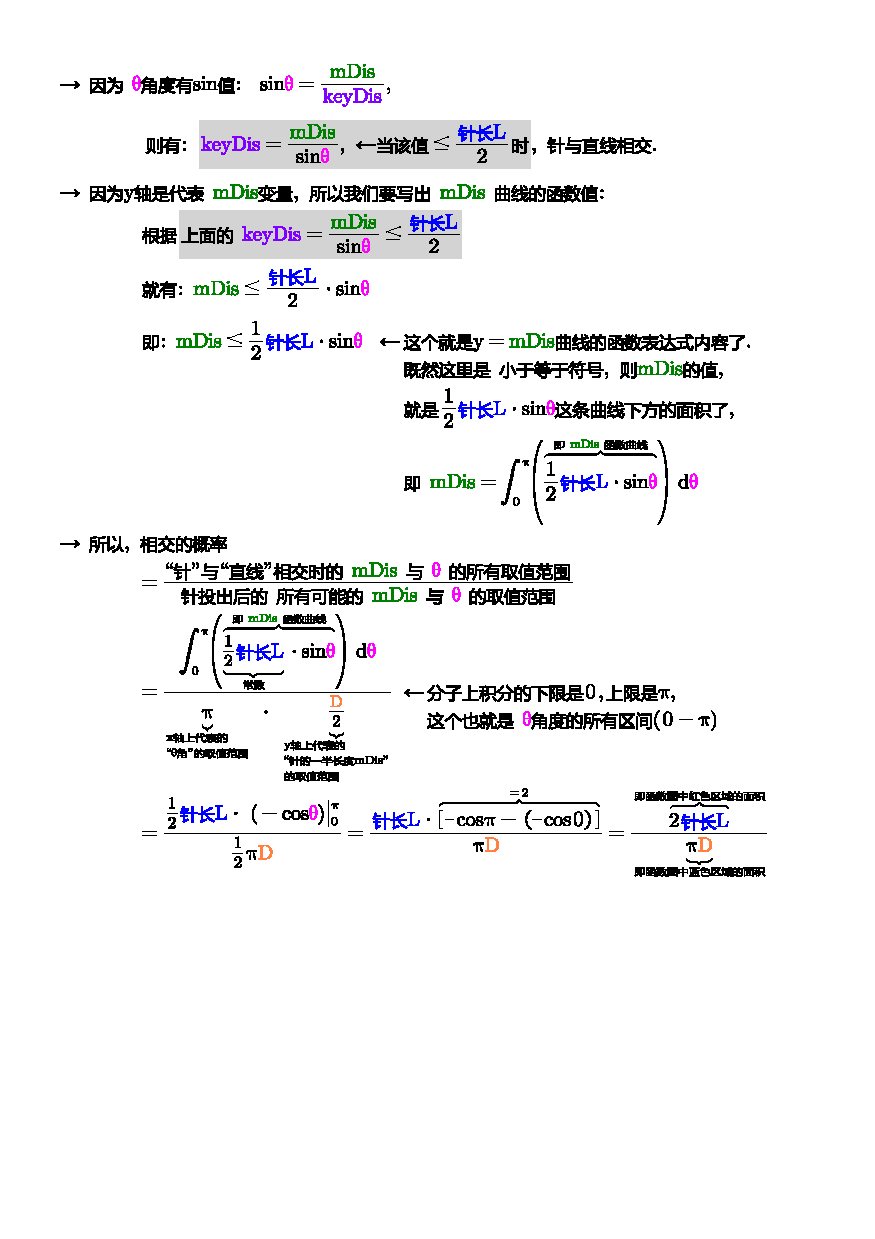
\includegraphics[width=0.97\textwidth]{/0085.pdf}
		
		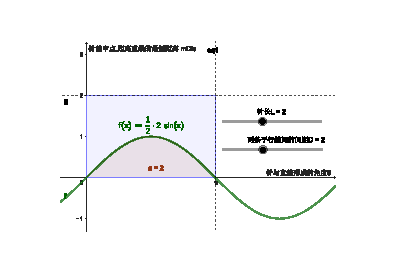
\includegraphics[width=0.8\textwidth]{/0087.pdf}
	\end{myEnvSample} 
	
	
	
	
	
	
	\section{``古典概率模型"和``几何概率模型"的区别}
	
	- 古典概率模型 : \\
	具有 ``有限可加性" (finite additivity): 是指``有限个"两两互不相容事件的``和事件"的概率, 等于``每个事件概率"的和. \\
	即: $
	\underset{\text{的概率}}{\underbrace{\text{P}\underset{\text{和}}{\underbrace{\left( \text{∪}_{\text{i}=1}^{\text{n}}\text{A}_{\text{i}} \right) }}}}=\underset{\text{的和}}{\underbrace{\sum_{\text{i}=1}^{\text{n}}{\underset{\text{概率}}{\underbrace{\text{P}\left( \text{A}_{\text{i}} \right) }}}}}
	$ \\
	\\
	
	- 几何概率模型 : \\
	具有``完全可加性":  即先求和, 再求概率, 等于 先求每个事件概率, 再求和. \\
	即: $
	\underset{\text{的概率}}{\underbrace{\text{P}\underset{\text{和}}{\underbrace{\left( \text{∪}_{\text{i}=1}^{\infty}\text{A}_{\text{i}} \right) }}}}=\underset{\text{的和}}{\underbrace{\sum_{\text{i}=1}^{\infty}{\underset{\text{概率}}{\underbrace{\text{P}\left( \text{A}_{\text{i}} \right) }}}}}
	$ \\
	
	注意两者的区别: 一个是``有限(到n)"的加,  一个是``无限(到∞)"的加.
	
	
	
	
	
	
\end{document}